\documentclass{standalone}
\usepackage{tikz}
\usetikzlibrary{intersections, calc}
\usepackage{hsbcommon}
    \begin{document}
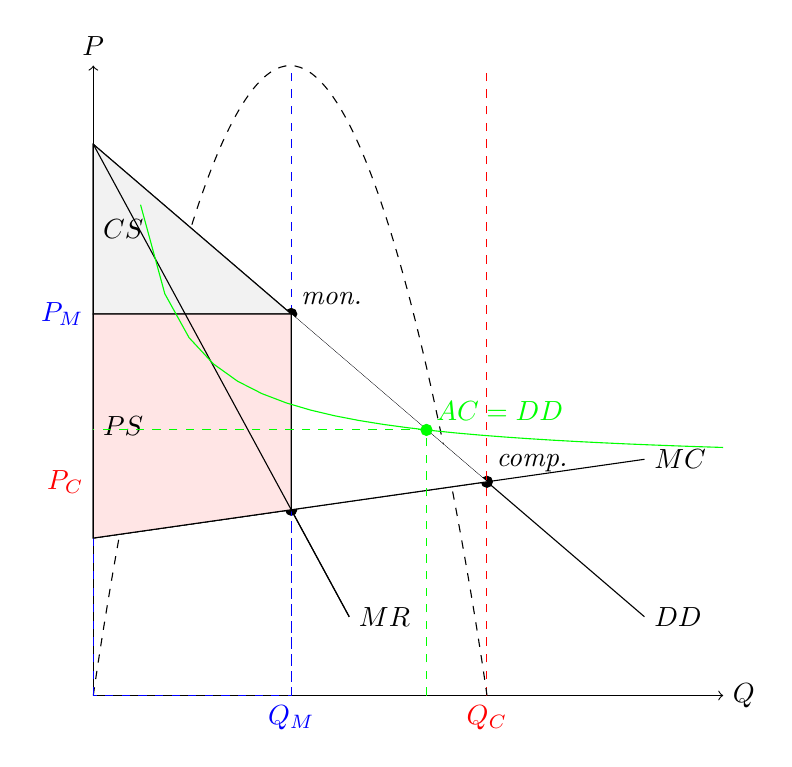
\begin{tikzpicture}[remember picture]
        \draw[->] (0,0) node[below] {\phantom{$X_i$}} -- (8,0) node[right] (Q) {$Q$};
        \draw[->] (0,0) node[left] {\phantom{$Y_mi$}} -- (0,8) node[above] (P) {$P$};

        \coordinate (A) at (0,7);
        % \coordinate (B) at (2,6);
        % \coordinate (C) at (3,4);
        % \coordinate (D) at (4,3);
        % \coordinate (E) at (6,2);
        \coordinate (F) at (7,1);
 
        \draw [name path=demand] plot [smooth] coordinates {(A) (F)};
        \node[right] at (F) {$DD$};

        % Demand curve

        \coordinate (G) at (0,2);
        % \coordinate (H) at (2,3);
        % \coordinate (I) at (3,3);
        % \coordinate (J) at (5,3);
        % \coordinate (K) at (6,3);
        \coordinate (L) at (7,3);
        
        \draw [name path=supply] plot [smooth] coordinates {(G) (L)};
        % \draw [name path=supply,domain=0:8] plot (\x,0.1*\x+2);
        \node[right] at (L) {$MC$};
        

        \ifstep{1}{
        
        %% COMPETITION CASE
            
            \path [name intersections={of=demand and supply,by=X}];
    
            \filldraw (X) circle (2pt) node[above right] {\textit{comp.}};
    
            % \draw[dashed, red] (0,0) rectangle (X);
            
            \draw [dashed,red ] (X |-, 0) node[below] {$Q_C$}-- (X |-, 8);
            \draw[red, dotted] (X) -- (0, |- X) node[left] {$P_C$};

            \draw [fill=blue!10] (X) -- (0, |- X) -- node [right] {$CS$}   (A);
            \draw [fill=red!10] (X) -- (0, |- X) -- node [right] {$PS$}  (G);
            
        }

        \ifstep{2}{

        %% MONOPOLY CASE
        
            % \coordinate (M) at (0,8);
            % \coordinate (B) at (2,6);
            % \coordinate (C) at (3,4);
            % \coordinate (D) at (4,3);
            % \coordinate (E) at (6,2);

            %% draw profit parablola
            \coordinate (M) at (0,0) ;
            \coordinate (N) at (2.5,8);
            \coordinate (O) at (5,0);
            \draw[dashed] (M) plot [smooth,tension=1] coordinates {(M) (N) (O)};
            
            \coordinate (N) at (3.25,1);
     
            \draw [name path=mr] plot [smooth] coordinates {(A) (N)};
            \node[right] at (N) {$MR$};
    
            \path [name intersections={of=mr and supply,by=Y}];
            \filldraw (Y) circle (2pt) node[above right] {\textit{Y}};
    
            \draw [name path=mono, dashed,blue ] (Y |-, 0) node[below] {$Q_M$} -- (Y |-, 8);
            \path [name intersections={of=mono and demand,by=Z}];
            
            \filldraw (Z) circle (2pt) node[above right] {\textit{mon.}};
            \draw[blue, dotted] (Z) -- (0, |- Z) node[left] {$P_M$};
    
        }

        \ifstep{3}{

            
            \draw [fill=white] (X) -- (G) -- (A);
            \draw[dashed, blue] (0,0) rectangle (Y);
            
            \draw [fill=gray!10] (Z) -- (0, |- Z) -- node[right] {$CS$} (A) --  cycle;
            
            \draw [fill=red!10]  (0, |- Z) --  (Z) --  (Y) --  (G) -- node[right] {$PS$}  cycle;

            \draw [name path=mr] plot [smooth] coordinates {(A) (N)};

        }

        %%% Average Cost Curve
        \ifstep{4}{
\begin{scope}[color=green]

            \draw [name path=averagecosts,domain=0.6:8,color=green] plot (\x,{(0.1*\x+2)/\x+2.8});
            \path [name intersections={of=averagecosts and demand,by=MONO}];
            \filldraw (MONO) circle (2pt);
            \draw[dashed] (MONO |-, 0) -- (MONO) -- (0, |- MONO);
            \node[above right] at (MONO) {$AC=DD$};
        \end{scope}
}

        
        
    \end{tikzpicture}
\end{document}
